\chapter{Reachable type analysis}
\label{chap:rta}
\section{Semantics}
In order to write a static analysis for determining a reachable type set, we first need to define what \emph{reachable types} are: the set of types actually reachable from some object at runtime.
\begin{definition}
\label{def:rts}
The \emph{reachable type set} $\mathcal{RTS} = \mathcal{JT} \mapsto \mathcal{P}$ is defined as a partial function from Java types $\mathcal{JT}$ to heap paths $\mathcal{P}$.
In addition to the operations on partial functions (see \cref{def:partial}) we define the following operations on reachable type sets:
\begin{itemize}
    \item The sum of two reachable type sets $s_1, s_2 : \mathcal{RTS}$ is defined by \[ s_1 + s_2 := s_1 \oplus s_2 \cup \{ \mathit{ty} \to s_1(\mathit{ty}) | s_2(\mathit{ty}) \ |\ \mathit{ty} \in \Dom(s_1 \cap s_2) \} \]
    \item Given a path $p : \mathcal{P}$ and a reachable type set $s : \mathcal{RTS}$ the type set with prepended path $p.s$ is defined by \[ p.s :=  \{ t \to p.s(t)\ |\ t \in \Dom(s) \} \]
    \item Analogous the type set with appended path $s.p$ is given by \[ s.p :=  \{t \to s(t).p\ |\ t \in \Dom(s) \} \]
    \item The operation $\Matching : (\mathcal{RTS}, \mathcal{H}^*) \to \mathcal{RTS}$ returns the reachable type set after accessing a sequence of heap edges and is defined by
    \[ 
    \Matching(s, hs) := \{ t \to p' \ |\ t \in \Dom(s), s(t) \equiv hs.p' \}
    \]
\end{itemize}
\end{definition}
For the definition of runtime reachable types we require an exact representation of heap sequences; this is provided by \emph{exact reachable type sets}.
\begin{definition}
An \emph{exact reachable type set} $\mathcal{RTS}_\text{exact} = \mathcal{JT} \mapsto \mathscr{P}(\mathcal{H}^*)$ is a variant of reachable type sets used for theoretical considerations of runtime reachable types that replaces the overapproximating heap path $\mathcal{P}$ with a set of exact heap sequences $\mathscr{P}(\mathcal{H}^*)$. 
\begin{itemize}
    \item The sum of two exact reachable type sets $s_1, s_2 : \mathcal{RTS}_\text{exact}$ is defined by \[ s_1 + s_2 := s_1 \oplus s_2 \cup \{ \mathit{ty} \to s_1(\mathit{ty}) \cup s_2(\mathit{ty}) \ |\ \mathit{ty} \in \Dom(s_1 \cap s_2) \} \]
    \item Given a heap sequence $h : \mathcal{H}^*$ and an exact reachable type set $s : \mathcal{RTS}_\text{exact}$ the type set with prepended path $p.s$ is defined by \[ h.s :=  \{ t \to \{h.h_s\ |\ h_s \in s(t) \}\ |\ t \in \Dom(s) \} \]
    \item Analogous the type set with appended heap sequence $s.h$ is given by \[ s.h := \{ t \to \{h_s.h\ |\ h_s \in s(t) \}\ |\ t \in \Dom(s) \} \]
    \item The operation $\Matching : (\mathcal{RTS}_\text{exact}, \mathcal{H}^*) \to \mathcal{RTS}_\text{exact}$ returns the exact reachable type set after accessing a sequence of heap edges and is defined by
    \[ 
    \Matching(s, h) := \{ t \to hs \ |\ t \in \Dom(s),  hs = \{ h'\ |\ h.h' \in s(t) \}, |hs| > 0 \}
    \]
\end{itemize}
\end{definition}
With $\mathcal{RTS}_\text{exact}$ we can then define the theoretical reachable types of a reference at runtime.
\begin{definition}[Runtime reachable types]
\label{def:rrt}
Let $\mathcal{RT}_c : \mathit{Refs} \to \mathcal{RTS}_\text{exact}$ denote the exact reachable type set of some reference with the memory state $c$ (i.e. register, stack, and heap content) and $\operatorname{class}(r)$ be the most specific class of the object referenced by $r$. The fields of a class $\mathit{cls}$ are denoted as $\mathcal{F}(\mathit{cls})$ and the size of the array referenced by $r_a$ is $|r_a|$. Then $\mathcal{RT}_c$ is defined as follows where $r$ denotes a reference to a class and $r_a$ an array reference:
\begin{align*}
    \mathcal{RT}_c(r) &:= \{ \operatorname{class}(r) \to \{ \epsilon \} \} + \sum_{f \in \mathcal{F}(\operatorname{class}(r))} f.\mathcal{RT}_c(r.f) \\
    \mathcal{RT}_c(r_a) &:= \sum_{i=0}^{|r_a|} i.\mathcal{RT}_c(r[i])
\end{align*}
\end{definition}
\begin{remark}
In case we encounter an cyclic reference such as in
\begin{javacode}
List xs = new List();
xs.next = xs;
\end{javacode}
we have an infinite heap sequence set for \texttt{xs}
\[ \{ \mathtt{List} \to \{ \epsilon, \mathtt{next}, \mathtt{next.next}, \cdots\} \} \]
\end{remark}

\begin{remark}
The runtime reachable types are exact. For all $r : \mathit{Refs}$ and heap sequences $path$ starting from $r$, the following holds: \[ \Matching(RT_c(r),path) = RT_c(r.path) \]
\end{remark}


\section{Flow analysis}
Our reachable type analysis is implemented as a Soot forward data flow analysis on a control-flow graph, returning a parametric method result that can be instantiated with varying argument sets. As the reachable types analysis requires analysis results of all invoked methods, each result is stored in a map of methods to analysis results. If a new method has to be analysed, the analysis is performed recursively and the result is added to the map for future use.

\begin{definition}
\label{def:pts}
A \emph{parametric type set} $\mathcal{PTS} = (\mathcal{RTS}, \mathbb{N} \mapsto \mathcal{P})$ is a 2-tuple of a reachable type set $\mathcal{RTS}$ as defined in \cref{def:rts} and a partial function $\mathbb{N} \mapsto \mathcal{P}$ from the natural numbers to heap paths used for storing placeholders for arguments where the heap path describes where the reference to the argument is reachable.
\begin{itemize}
    \item The sum $\mathit{pts}_1 + \mathit{pts}_2 : \mathcal{PTS}$ of two parametric type sets $\mathit{pts}_1, \mathit{pts}_2 : \mathcal{PTS}$ is defined as 
    \begin{align*}
    (\mathit{rts}_1, p_1) + (\mathit{rts}_2, p_2) :=&\ (\mathit{rts}_1 + \mathit{rts}_2, p_1 \oplus p_2\ \cup \\
        &\ \{ n \to p_1(n) | p_2(n) \ |\ n \in \Dom(p_1 \cap p_2) \})
    \end{align*}
    \item The function $\operatorname{apply} : (\mathcal{PTS}, \mathcal{PTS}^*) \to \mathcal{PTS}$ is used to simulate the effects of a method invoke on the parametric type set. It is passed a sequence of parametric type sets for each passed argument and returns the updated parametric type set. The definition is 
    \[
    \operatorname{apply}((rts, ps), args) :=  (rts, \varnothing) + \sum_{n \in \Dom(ps)} ps(n).args_n
    \]
\end{itemize}
\end{definition}
\begin{example}
The application of a parametric type set $pts$, given by \[ pts = (\{\mathtt{List} \to \{\mathtt{next}^{[0,*]}\}\}, \{0 \to \epsilon, 2 \to \mathtt{value}\})\] to a sequence of arguments $\mathit{args}$ defined by \[\mathit{args} = ((\varnothing, \varnothing), (\varnothing, \varnothing), (\{ \texttt{Object} \to \epsilon \}, \varnothing))\] is the following parametric type set \[ \operatorname{apply}(pts, \mathit{args}) = (\{\mathtt{List} \to \{\mathtt{next}^{[0,*]}\}, \mathtt{Object} \to \mathtt{value}\}) \]
\end{example}

\begin{definition}
\label{def:pmr}
A \emph{parametric method result} $\mathcal{PMR} = (\mathcal{PTS}, \mathcal{PTS}^*)$ is a 2-tuple consisting of 
\begin{enumerate}
    \item a parametric type set containing the return value's reachable types
    \item a sequence of parametric type sets with the updated arguments' reachable types
\end{enumerate}

\begin{itemize}
    \item The $\operatorname{apply} : (\mathcal{PMR}, \mathcal{PTS}^*) \to \mathcal{PMR}$ operator for method results is defined by applying the argument sets on each underlying set: \begin{align*}
\operatorname{apply}((\mathit{retPts}, \mathit{argsPts}), args) :=& (\operatorname{apply}(\mathit{retPts}, args), \\
    & (\operatorname{apply}(\mathit{argsPts}_i, args))_{i \in [0,|\mathit{argsPts}|]})
    \end{align*}
                \item The sum of two parametric method results for the same method $\mathit{pmr}_1, \mathit{pmr}_2 : \mathcal{PMR}$ is the sum of its components:
    
        \[ (r_1, a_1) + (r_2, a_2) := (r_1 + r_2, (a_{1,i} + a_{2,i})_{i \in [0, |a_1|]}) \]
    

\end{itemize}
\end{definition}
\begin{example}
\label{ex:pmr}
Consider the following Java code:
\begin{javacode}
public static List setValue(Object value, List xs) {
    xs.value = value;
    return xs;
}
\end{javacode}
Then the parametric method result for \text{List setValue(Object,List)} is \[( \underbrace{(\varnothing, \{ 0 \to \mathtt{value}, 1 \to \epsilon\})}_\text{return value type set} , (\underbrace{(\varnothing, \{0 \to \epsilon\})}_\text{first argument}, \underbrace{(\varnothing, \{ 0 \to \mathtt{value}, 1 \to \epsilon\})}_\text{second argument}))\]
\end{example}
\newpage
\begin{definition}
The \emph{control-flow graph} $G(m) = (V \subseteq \mathit{Stmt},E \subseteq V \times V)$ of a Jimple method $m$ is a directed graph where the vertices are the method's Jimple statements and there exists an edge $v_1 \to v_2$ iff execution can progress from $v_1$ to $v_2$. Its only source is the first statement of the Jimple method and its sinks are the return points.
\end{definition}
\begin{example}
To create a control-flow graph from Java code, it first has to be converted into Jimple statements.
\begin{javacode}
public Object constructList(Object x) {
    List orig = new List();
    List xs = orig;
    
    for (int i = 0; i < 100; i++) {
        if (x != null) {
            xs.value = x;
        } else {
            xs.value = new Unit();
        }

        xs.next = new List();
        xs = xs.next;
    }
    return orig;
}
\end{javacode}
The loop structure and \javainline{if}/\javainline{else} branch are easily recognizable and statements are fairly complicated. For analysis puproses, the Java code has to be transformed into Jimple code.
The following code is the Jimple equivalent of the Java code above. It can then be processed into a control-flow graph.
\pagebreak
\begin{minted}[linenos]{text}
public java.lang.Object constructList(java.lang.Object) {
    ListUtils r0;
    java.lang.Object r1;
    List r2, $r3, $r5, r6;
    Unit $r4;
    int i0;
    
    r0 := @this: ListUtils;
    r1 := @parameter0: java.lang.Object;
    
    $r3 = new List;
    specialinvoke $r3.<List: void <init>()>();
    
    r2 = $r3;
    r6 = r2;
    i0 = 0;
 label1:
    if i0 >= 100 goto label4;
    if r1 == null goto label2;
    r6.<List: java.lang.Object value> = r1;
    goto label3;

 label2:
    $r4 = new Unit;
    specialinvoke $r4.<Unit: void <init>()>();
    r6.<List: java.lang.Object value> = $r4;

 label3:
    $r5 = new List;
    specialinvoke $r5.<List: void <init>()>();
    r6.<List: List next> = $r5;
    r6 = r6.<List: List next>;
    i0 = i0 + 1;
    goto label1;

 label4:
    return r2;
}
\end{minted}
As we can see, our high-level Java code with a \javainline{for}-loop got transformed into unnested code reminiscent of Java bytecode and assembly. The \javainline{for}-loop became a flat construct:
\begin{minted}[linenos]{text}
label1:
    if i0 >= 100 goto label4;
    // loop body
    i0 =  i0 + 1;
    goto label1;
label4:
    return r2;
\end{minted}
Similarly, the \javainline{if}/\javainline{else} statement also became a series of \texttt{goto}s:
\begin{minted}[linenos]{text}
if r1 == null goto label2;
// if body
goto label3;
label2:
// else body
label3:
// remainder
\end{minted}
Note that there are some dissimilarities with Soot's Jimple output and our Jimple syntax. \emph{External} Jimple output includes method and variable declarations which are not part of the actual Jimple statements and thus also not included in the control-flow graph.
\begin{minted}{text}
public java.lang.Object constructList(java.lang.Object) {
    ListUtils r0;
    java.lang.Object r1;
    List r2, $r3, $r5, r6;
    Unit $r4;
    int i0;
    // ...
}
\end{minted}
The resulting control-flow graph is given below:\\
\pagebreak
\includegraphics[scale=0.85]{CFG.eps}
\end{example}
Here we can see the branches and loop structure again that became less obvious in the Jimple code, such as the loop structure in \cref{fig:cfg-for} or the branch structure in \cref{fig:cfg-ifelse}.
\begin{figure}[ht]
    \centering
    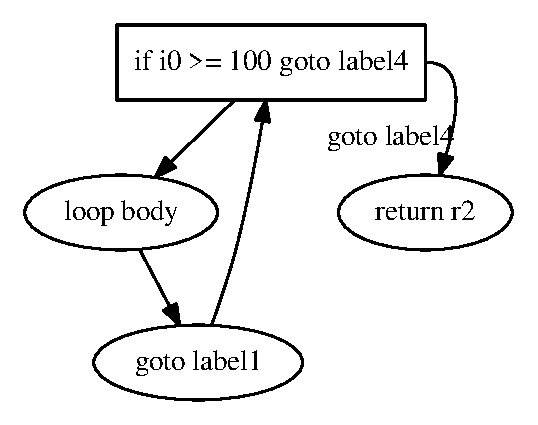
\includegraphics{CFG-for.eps}
    \caption{For loop in the control-flow graph}
    \label{fig:cfg-for}
\end{figure}

\begin{figure}[ht]
    \centering
    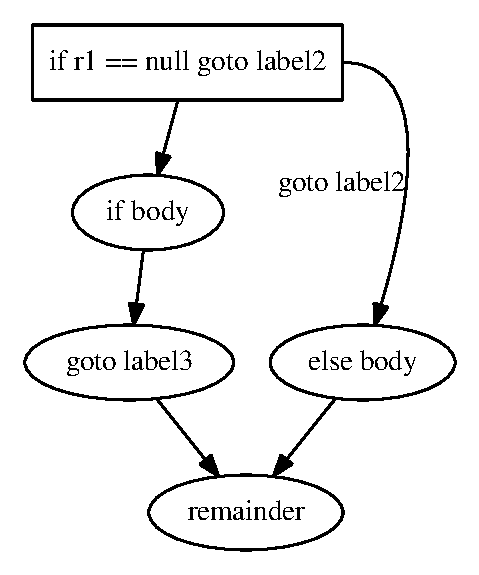
\includegraphics{CFG-ifelse.eps}
    \caption{If/else branch in the control-flow graph}
    \label{fig:cfg-ifelse}
\end{figure}
\pagebreak

\begin{definition}[Possible types of a right-hand value]\label{def:pt}
Given two partial functions $a, b : \mathit{Refs} \mapsto \mathcal{PTS}$ where $a$ is the analysis state before the current statement and $b$ is the new state and a Jimple \emph{rvalue} (see \cref{subsect:jimple}), the function $\operatorname{pt} : (\mathit{Refs} \to \mathcal{PTS})^2 \times \mathit{rvalue} \to \mathcal{PTS}$ is defined by performing case analysis on the \emph{rvalue}:
\begin{case}
    \item[Local variables and static fields] For local variables and static fields, return the previous set in $a$. This set is always defined as uninitialised variables cannot occur.
    
    \item[Instance fields and array accesses] For instance field accesses \texttt{r0.value} or array accesses \texttt{r0[idx]} retrieve the preceding type set $pts$ for \texttt{r0} from $a$ and return $\Matching(pts, \texttt{value})$ respectively $\Matching(pts, \texttt{arrayAccess})$. If there is no matching type set, then use the empty type set as the field is \texttt{null} if it never occurred in the base local's type set.
    
    \item[\emph{invokeExpr}] Invoke expressions are handled differently based on whether static or dynamic dispatch is used.
    For \texttt{specialinvoke} and \texttt{staticinvoke}, static dispatch is used; analysing the invoke target is sufficient.
    
    However for dynamic invokes (\texttt{interfaceinvoke} and \texttt{virtualinvoke}), all possible concrete subclasses of the target method's class have to be analysed, with the results added together: If the type set of the base local contains a placeholder, analyse all possible implementations; otherwise it is sufficient to analyse the types whose paths match $\epsilon$.
    
    A reachable type analysis is performed on the invoked method (or a previously computed method result is retrieved), instantiating it with the invoke arguments' type sets. The result is then used to update the values and heap-shape predecessors of the passed arguments' sets like in the \emph{assignStmt} case in \cref{def:flowThrough}, and the return set is used as the returned result.
    
    \item[\emph{castExpr}] The cast's underlying reference's set is returned.
    
    \item For all other expressions such as \texttt{new}, \texttt{instanceof} and so on, the type of the expression is returned.
\end{case}
\end{definition}

\begin{example}
\label{ex:pt}
We consider the possible types of a right-hand value after the first 3 statements in this method execute:
\begin{javacode}
public void example() {
    List xs = new List();
    xs.value = new Unit();
    Object obj = this;
}
\end{javacode}
The state after line 4 is then \[ a := \{\mathtt{xs} \to (\{\mathtt{List} \to \epsilon,\ \mathtt{Unit} \to \mathtt{value} \}, \varnothing), \mathtt{thing} \to (\varnothing, \{ 0 \to \epsilon \}) \}\] and $b := a$.
The possible types for different right-hand values after line 3 are then:
\begin{align*}
    \operatorname{pt}(a,b,r_0) &= (\{ \mathtt{List} \to \epsilon,\ \mathtt{Unit} \to \mathtt{value} \}, \varnothing)\\
    \operatorname{pt}(a,b,r_0.\mathtt{value}) &= (\{ \mathtt{Unit} \to \epsilon \}, \varnothing)\\
    \operatorname{pt}(a,b,\mathtt{setValue}(\mathtt{obj}, \mathtt{xs})) &= (\{ \mathtt{List} \to \epsilon,\ \mathtt{Unit} \to \mathtt{value} \}, \{ 0 \to \mathtt{obj} \}) \\
    \text{with } b &= \{ \mathtt{xs} \to (\{ \mathtt{List} \to \epsilon,\ \mathtt{Unit} \to \mathtt{value} \}, \{ 0 \to \mathtt{value} \})\\
    &\ \ \  ,\  \mathtt{obj} \to (\varnothing, \{ 0 \to \epsilon \}) \} \\
    \operatorname{pt}(a,b,\mathtt{new\ Object}) &= (\{ \mathtt{Object} \to \epsilon \}, \varnothing)
\end{align*}
where the parametric method result for $\mathtt{setValue}$ is computed in \cref{ex:pmr}.
\end{example}

The flow-through function is used to propagate the state along the control-flow graph.
\begin{algorithm}[Flow-through function]
\label{def:flowThrough}
The function $\operatorname{flowThrough} : (\mathit{Refs} \mapsto \mathcal{PTS}, \mathit{Stmt}) \to \mathit{Refs} \mapsto \mathcal{PTS}$ is defined for $a : \mathit{Refs} \mapsto \mathcal{PTS}$ and $stmt : \mathit{Stmt}$ as follows:
\begin{enumerate}
    \item Initializing the new state with the preceding state $b := a$
    \item Performing case analysis on the $stmt$:
        \begin{case}
            \item[\emph{assignStmt}] If we have an \emph{assignStmt}, which has the form \texttt{x = y}, use \cref{def:pt} to calculate the possible types $\mathit{rvPts} = \operatorname{pt}(a, b, y)$ of the \emph{rvalue} \texttt{y}. 
            \begin{enumerate}[label=\textbf{Case 1.\arabic*:}, itemindent=*]
                \item[\texttt{x} is a local variable] If \texttt{x} is a local variable, just set $b(\mathtt{x}) = \mathit{rvPts}$
                \item[\texttt{x} is a field or array reference] Otherwise \texttt{x} is a field or array reference. This case causes heap data to change, requiring us to take heap shape into account.
                    Using the heap-shape analysis we calculate all predecessors of \texttt{x}, giving us a partial function $\mathit{preds} : \mathit{Refs} \mapsto \mathcal{P}$ from references to paths. Then for each $v \in \Dom(\mathit{preds})$, $b(v) = b(v) + \mathit{preds}(v).\mathit{rvPts}$
            \end{enumerate}
            \item[\emph{identityStmt}] For an \emph{identityStmt} \texttt{local = @this} or \texttt{local = @parameter}$n$, set $b(\texttt{local}) = (\varnothing, \{idx \to \epsilon\})$ where $idx = 0$ in the \texttt{@this} case, $n$ in the \texttt{@parameter}$n$ case when the method being analysed is static, or $n+1$ otherwise.
            \item[\emph{invokeStmt}] An \emph{invokeStmt} consists solely of an \emph{invokeExpr}. This case is handled by invoking $\operatorname{pt}(a, b, \mathit{invokeExpr})$.
        \end{case}
    \item Return $b$.
\end{enumerate}
\end{algorithm}

We require a framework in which we can apply our flow-through function. This is provided by the forward data flow analysis, which applies the flow-through function to every node of the control flow graph.
\begin{algorithm}[Forward data flow analysis]
\label{def:fdfa}
Given a control-flow graph $(V \subseteq \mathit{Stmt},E)$ the \emph{forward data flow analysis} creates two partial functions $a, b : \mathit{Stmt} \mapsto \mathit{Refs} \mapsto \mathcal{PTS}$ where $a$ is the analysis state before the given statement and $b$ is the state after. The analysis is performed by traversing the graph starting at the entry point. For each $\mathit{stmt} \in V$:
\begin{case}
    \item[$a(\mathit{stmt})$ undefined] If $a(\mathit{stmt})$ is undefined, we're at the entry point. Set $a(\mathit{stmt}) := \varnothing$ and go to case 2.
    \item[$b(\mathit{stmt})$ undefined] If $b(\mathit{stmt})$ is undefined, the node hasn't been examined yet. \\Set $b(\mathit{stmt}) = \operatorname{flowThrough}(a(\mathit{stmt}), stmt)$.
    \item If both functions are defined at $\mathit{stmt}$, we perform a fixpoint iteration by setting $b(\mathit{stmt}) = flowThrough(a(\mathit{stmt}),\mathit{stmt})$. If this did not cause a change in $b(\mathit{stmt})$, we remove all predecessors of $\mathit{stmt}$ from the control-flow graph to stop the fixpoint iteration.
\end{case}

After we set $b(\mathit{stmt})$, we need to update the partial function $a$ for all successors $\operatorname{succ}(\mathit{stmt})$: For all $\mathit{next} \in \operatorname{succ}(\mathit{stmt})$:
\begin{case}
    \item[$a(\mathit{next})$ undefined] If $a(\mathit{next})$ undefined, set $a(\mathit{next}) = b(\mathit{stmt})$
    \item Otherwise, set $a(\mathit{next}) = a(\mathit{next}) + b(\mathit{stmt})$
\end{case}
We do not need to iterate manually, as loops in the control-flow graph already cause iterations.
\end{algorithm}
\begin{example}
Using the code for \texttt{setValue}, we can now derive how the state after each line is computed. The \javainline{example()} method consists of the following Jimple statements:
\begin{minted}[linenos]{text}
r0 = @this;
r1 = new List;
specialinvoke r1.<init>();
r2 = new Unit;
specialinvoke r2.<init>();
r1.value = r2;
r3 = r0;
\end{minted}

For simplicity, let $s_n$ denote the statement at line $n$. The initial state $a(s_0)$ is empty. Applying the flow-through function to determine $b(s_0) = \operatorname{flowThrough}(a(s_0), s_0)$ we can see that the \emph{identityStmt} case is chosen. Thus $b(s_0) = \{ \texttt{r0} \to (\varnothing, \{ 0 \to \epsilon \}) \}$. Then we set $a(s_1) = b(s_0)$ and continue. 

Calculating $b(s_1) = \operatorname{flowThrough}(a(s_1), s_1)$ the \emph{assignStmt} case in $\operatorname{flowThrough}$ is used. Then $\operatorname{pt}(a(s_1), b(s_1), \texttt{new List}) = (\{ \mathtt{List} \to \epsilon \}, \varnothing)$  and $b(s_1) = b(s_0) + \{ \mathtt{r1} \to (\{ \mathtt{List} \to \epsilon \}, \varnothing) \}$

The constructors of \texttt{List} and \texttt{Unit} are empty, leading to $b(s_3) = a(s_3)$ and $b(s_5) = a(s_5)$. For $s_4$ the procedure is identical to $s_2$, leading to $b(s_4) = b(s_3) + \{ \mathtt{r2} \to (\{ \mathtt{Unit} \to \epsilon \}, \varnothing) \}$

Finally after $s_7$ we have state 
\begin{align*}
    b(s_7) &= \{ \texttt{r0} \to (\varnothing, \{ 0 \to \epsilon \}), \texttt{r1} \mapsto (\{ \mathtt{List} \to \epsilon \}, \varnothing)\\
    &\ \ \ ,\ \texttt{r2} \mapsto (\{ \mathtt{Unit} \to \epsilon \}, \varnothing),  \texttt{r3} \to (\varnothing, \{ 0 \to \epsilon \}) \}
\end{align*}
\end{example}
We require a summary of the effects a method invocation has. This is given by the \emph{parametric method result} from \cref{def:pmr}.
\begin{definition}[Method result]
After performing the forward data flow analysis on a method with control-flow graph $(V,E)$ with result $a, b : \mathit{Stmt} \mapsto \mathit{Refs} \mapsto \mathcal{PTS}$, a method result for the return points $s_r \in \operatorname{sinks}(V,E)$ is a parametric method result consisting of:
\begin{enumerate}
    \item The parametric type set at $b(s_r)$ for the returned reference, or the empty set if the function returns void
    \item A sequence of sets at $b(s_r)$ for \texttt{this} and all arguments
\end{enumerate}
The actual method result is then the sum of all individual method results.
\end{definition}
\begin{example}
\label{ex:branch}
Given the following Java method with two return statements where in the first branch, only \texttt{String} is reachable and in the other branch the whole type set of argument $x$
\begin{javacode}
public Object removeNull(Object x) {
    if (x == null) {
        return new Nothing();
    } else {
        return x;
    }
}
\end{javacode}
the analysis result has to include both \texttt{Nothing} and the type set for \texttt{x}, as statically analysing which branch to choose is generally impossible here.
\end{example}

\section{Correctness}
\begin{theorem}
The reachable type analysis is sound modulo static fields---all types that a reference can possibly reach during the execution of a program are computed by the flow analysis as long they do not involve static fields across method boundaries.
\end{theorem}
\begin{proof}{Proof sketch}
Consider the control-flow graph $(V,E)$ of a method $m$ and let $a, b : \mathit{Stmt} \mapsto \mathit{Refs} \mapsto \mathcal{PTS}$ be the results of the forward data flow analysis on $(V,E)$. For all statements $s \in V$ let $c(s)$ be the memory state directly after executing $s$ and $\mathcal{RT}_{c(s)}$ the actual reachable types at the memory state $c(s)$ as in \cref{def:rrt}. Furthermore we require a sequence of method argument type sets $\mathit{args} : \mathcal{RTS}^*$ so that if $m$ is a n-ary method (counting \texttt{this} as an argument), $s_0 := r_0 = \texttt{@this}$ or $s_i :=  r_i = \texttt{@parameter}i$ if $m$ is static, $s_{i+1} := r_{i+1} = \texttt{@parameter}i$ otherwise,  $|\mathit{args}| = n$ and $\forall i \le n, \mathcal{RT}_{c(s_i)}(r_i) \subseteq \mathit{args}_i$. This ensures that we can instantiate all parametric type sets to a fully concrete reachable type set while maintaining soundness.
Then for all references $r$ in $\Dom(b(s))$ the proposition $\mathcal{RT}_{c(s)}(r) \subseteq \mathit{rts}$ with $(rts, \varnothing) = \operatorname{apply}(b(s)(r), \mathit{args})$ has to hold in order for the analysis to be sound.

Note that $f \subseteq g$ for $f : \mathcal{RTS}_\text{exact}$, $g : \mathcal{RTS}$ is defined as follows:
\[ f \subseteq g := \forall \mathit{ty} \in \Dom(f), \mathit{ty} \in \Dom(g) \land \forall h \in f(\mathit{ty}), h \Downarrow g(\mathit{ty}) \]
Informally, the idea is that a set of heap sequences matches a heap path iff they all match---similar to path equivalence.

We perform induction on the construction of $\mathcal{RT}_{c(s)}(r)$
\begin{case}
    \item[Base: $\mathcal{RT}_{c(s)}(r) = \varnothing$] Trivial.
    \item[Step: $\mathcal{RT}_{c(s)}(r) = R \cup \{ \texttt{cls} \to hs \}$ with $R \subseteq \mathit{rts}$] As $R \subseteq \mathit{rts}$ by induction hypothesis, it remains to prove that $\{ \texttt{cls} \to hs \} \subseteq \mathit{rts}$. First we consider the non-cyclic subset of $hs$. Then for all $h \in hs$ there exists a decomposition of the form $h=h_1.\cdots.h_n$ and a statement structure of the form
    \begin{minted}{text}
    rhn = new cls;
    ...
    rh1.h2 = rh2
    ralias.field = rh1
    r.h1 = ralias.field
    \end{minted}
    or
    \begin{minted}{text}
    rhi = @parameter //some identityStmt
    ...
    rh1.h2 = rh2
    ralias.field = rh1
    r.h1 = ralias.field
    \end{minted}
    where \texttt{ralias} is a placeholder for possible aliasing between each reference.
    \begin{enumerate}[label=\textbf{Case 2.\arabic*:},itemindent=*]
        \item[All statements were intraprocedual]
        If all statements were an \emph{assignStmt}, then the flow analysis follows each statement. The first statement's right-hand value $\operatorname{pt}(a,b,\texttt{new cls})$ results in a parametric type set $(\{ \texttt{cls} \to \epsilon \}, \varnothing)$ which is then propagated along the statements, with possible aliasing handled by the heap-shape analysis. As the heap-shape analysis is sound, we can conclude that $h \Downarrow b(s)(r)(cls)$
        
        If one of the statements was an \emph{identityStmt}, then by precondition on the argument type sets $\mathit{args}_i$, the possible types returned by $\operatorname{pt}(a,b,r_i)$---where $r_i$ is the local variable in the appropriate \emph{identityStmt} as defined above---should be eventually replaced by the correct type set. However \textbf{due to an error when modularising the analysis, this does not work properly for $r_i.\mathtt{field}$-type accesses.} In the non-parametric case for some reference $x$, the access $x.\mathtt{field}$ resolves to $(\varnothing, \varnothing)$ if no path matches \texttt{field}. This simulates the effect of an uninitialised field correctly on a non-parametric set, but not for parametric sets. A possible solution is given \cref{chap:future}---as this was only noticed during the final stages of the thesis there is insufficient time to provide a proper solution.
        \item[Some statements occur in an invoked method]
        In case the invoke is statically dispatched, the correct method is chosen every time. Otherwise for a dynamic invoke $b.m(...)$ and assuming soundness for $b$ then either all possible implementations out of the concrete reachable type set or all possible implementations period have been chosen, analysed and their method results added together.
        
        The method result is then applied to the type sets of the arguments, replacing all eventual placeholders local to the scope of the invoked method with placeholders local to the scope of the invoking method. The resulting return and updated argument type sets then (barring the bug with argument field accesses) propagate the type changes. As every possible method has contributed to the method result, the actually chosen method's effects are also represented in the parametric type sets.
    \end{enumerate}
    
    In case there exists a cyclic reference, $hs$ is infinite. However it has to be periodic, i.e. $hs$ is decomposable into a finite set of non-cyclic references $hs_\text{fin}$ and a finite set of 2-tuples $\mathit{cycles}$ consisting of a prefix $h_\text{pre}$ and an infinite set $hs_\text{suf}$ consisting of an iterated suffix $h_\text{suf}$
    so that \[ hs = hs_\text{fin} \cup \bigcup_{(h_\text{pre}, hs_\text{suf}) \in \mathit{cycles}} \bigcup_{h_\text{suf} \in hs_\text{suf}} h_\text{pre}.h_\text{suf}\]
    Then the cycle is created by an assignment of the form $r_0.f = r_1$ where $r_0$ is a successor of $r_1$. By soundness of the heap-shape analysis this statement causes all paths involving $r_0$ and $r_1$ to be adjusted for the infinite cycles by setting the upper bound on all constituent fields to $*$. 
    
    We can conclude that $cls \in \Dom(b(s))$ and $\forall h \in hs, h \Downarrow b(s)(cls)$.
    
    
\end{case}
\end{proof}
\begin{theorem}
The flow analysis tracks all execution paths that modify objects pointed to by references.
\end{theorem}
\begin{proof}[Proof sketch]
The intraprocedual case is trivial---this is handled by the control-flow graph. In case we encounter an \emph{invokeExpr}, the static dispatch cases always call the same statically known function, and thus are not particularly interesting.

The dynamic dispatch case however takes exactly one code path at runtime but it is not always possible to decide what code paths it will take at compile time.
If the method base object's type set contains any placeholders, it is not possible to determine exactly what subclass is called; thus, all subclass methods are analysed, including the actually used one.
If the type set doesn't contain any placeholder then due to soundness of the reachable type analysis we also have the actually used subclass in the type set.
\end{proof}
\begin{remark}
The analysis is not complete --- there can exist types in the type set that are unreachable during program execution; see \cref{ex:branch}.
\end{remark}